\section{Results}
\label{sec:exp}

Figure \ref{fig:results} shows the performance results obtained by the SVMs
in classification and regression for each subject and modality; Figure
\ref{fig:guess} shows four examples of predicted targets.

\begin{figure*}[!ht] \centering
  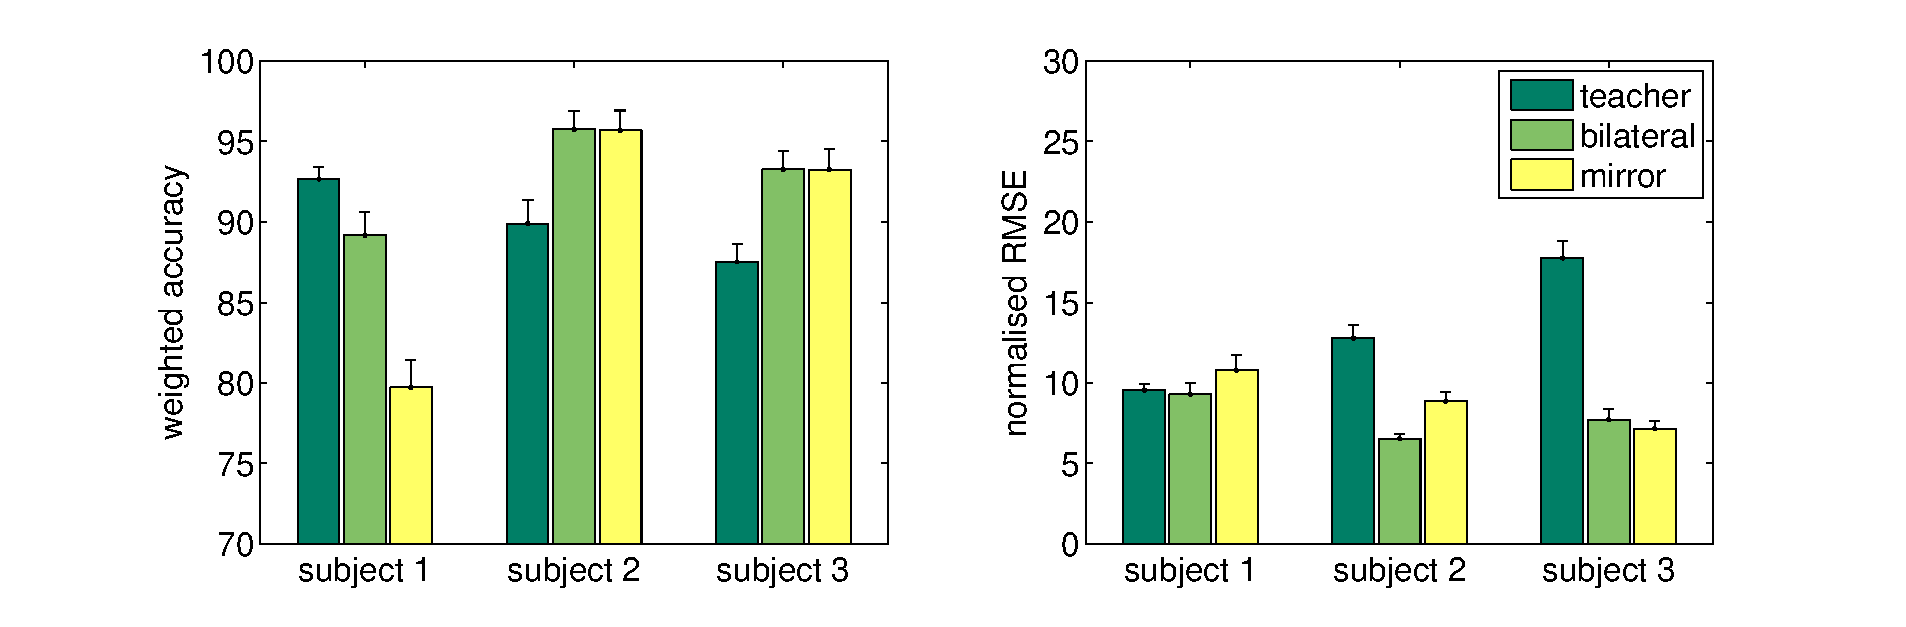
\includegraphics[width=\textwidth]{figs/figPerf}
  \caption{classification (left) and regression (right) performance
    for each subject and modality. Histogram bars are mean values over
    the $10$ splits of the outer cross-validation, error bars denote one
    standard deviation.}
  \label{fig:results}
\end{figure*}

Classification performance ranges from $95.74\% \pm 1.15\%$ (Subject $2$,
bilateral action) to $79.72\% \pm 1.70\%$ (Subject $1$, mirror-box). Highest
performances per subject are $92.67\% \pm 0.74\%$ (Subject $1$ in teacher
imitation modality), $95.74\% \pm 1.15\%$ (Subject $2$, bilateral action)
and $93.26\% \pm 1.11\%$ (Subject $3$, bilateral). Notice that
bilateral action and mirror-box are not significantly different as far as
Subjects $2$ and $3$ are concerned. A definite descending trend is observed
for Subject $1$ from imitation to bilateral to mirror-box, while this trend
is reversed for Subjects $2$ and $3$, which perform much better in the last
two modalities than in the first one. Modality-wise, teacher imitation is
the best modality for Subject $1$, while the other two are best for Subjects
$2$ and $3$.

Regression performance\footnote{Notice that the regression performance index
is an \emph{error}, while the classification performance is an \emph{accuracy};
therefore in the case of classification, the higher the bars, the better, whereas
it is the other way around in regression.} ranges from $6.54\% \pm 0.31\%$ (Subject $2$,
bilateral) to $17.76\% \pm 1.06\%$ (Subject $3$, teacher). Subject $1$ has
little or no significative difference among modalities, obtaining the best
performance while doing bilateral action ($9.29\% \pm 0.73\%$); Subject $2$
is best in bilateral action ($6.54\% \pm 0.31\%$) while Subject $3$ performs
best in mirror-box ($7.17\% \pm 0.43\%$) with high overlapping with the bilateral
modality. Subject-wise, Subjects $2$ and $3$ perform remarkably bad in teacher
imitation modality if compared with the other two; while modality-wise, we here
notice again that teacher imitation gets worse and worse as we move from Subject
$1$ to $2$ to $3$. A reversed trend is almost consistently observed for the other
two modalities.

\begin{figure*}[!ht] \centering
  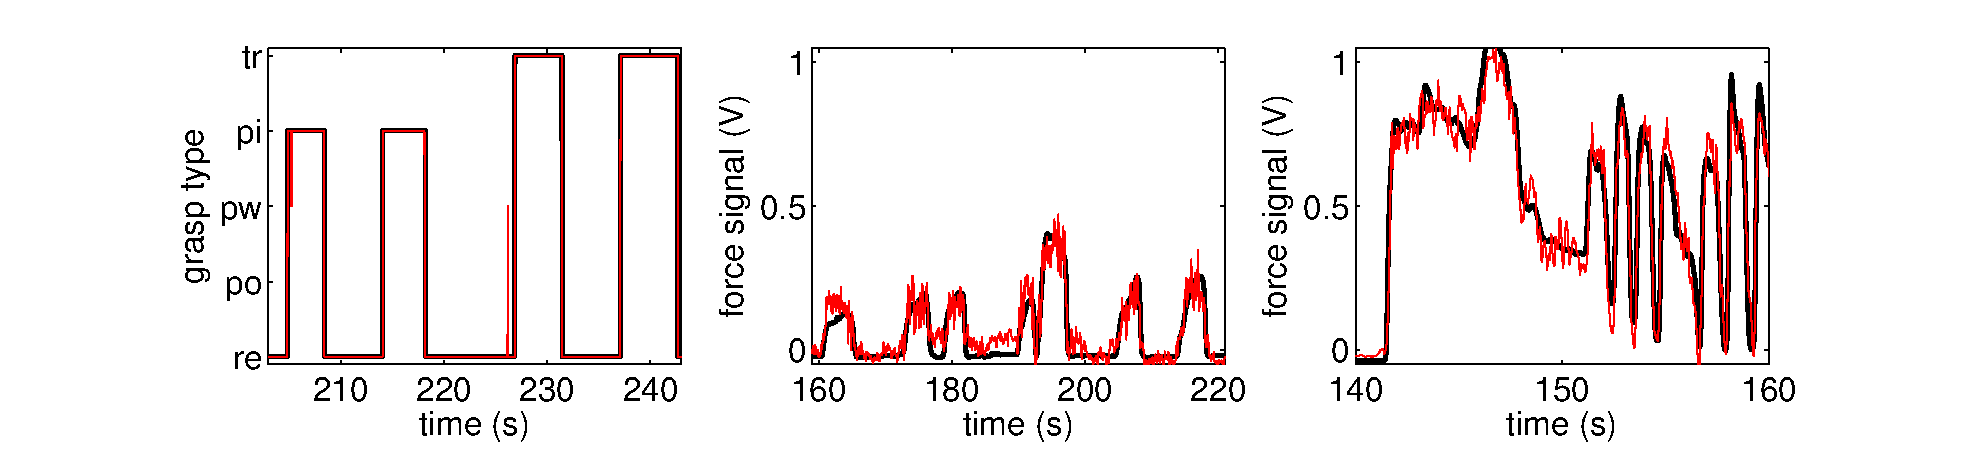
\includegraphics[width=\textwidth]{figs/figGuess}
  \caption{comparing true and predicted targets. (upper row) Classification
    of Subject $2$ in bilateral action (left, weighted accuracy $95.74\% \pm
    1.15\%$) and Subject $1$ in mirror-box (right, $79.72\% \pm 1.70\%$).
    (lower row) Regression of Subjects $2$ (left, normalised RMSE $6.54\% \pm
    0.31\%$) and $3$ (right, $7.70\% \pm 0.65\%$) in bilateral action.}
  \label{fig:guess}
\end{figure*}

Figure \ref{fig:guess} indicates that (upper row) most errors in classification
appear at the onset of grasps (transitions to/from label \re), although for Subject $1$
\pw\ and \pi\ are also frequently mistaken. Regression (lower row) appears good
both when force is approximated during slow (left panel) and fast (right panel)
grasps. The only significant disturbance is a high-frequency but low-amplitude
modulation of the predicted force. Confusion matrices for each subject and
modality (Figure \ref{fig:confusion}) actually confirm that \re\ is easily mistaken
for any other label (first row and column of each matrix), in particular for
Subjects $2$ and $3$. Subject $1$ has a more complex schema of label confusion,
depending on the modality. In particular, during teacher imitation, \pi\ and
\tr\ are easily confused; during bilateral action, \pi\ and \pw\ are as well
confused; and in mirror-box modality the pointing index and the power grasp
are those most easily mistaken. Actually, this is qualitatively confirmed by
considering again the PCA-reduced sample scatterplots of Figure \ref{fig:PCA},
first row.

\begin{figure*}[!ht] \centering
  \includegraphics[width=\textwidth]{figs/figConf}
  \caption{confusion matrices for each subject and modality.
    In each matrix $C$, $C_{ij}$ denotes the fraction of labels
    $i$ which have been mistaken for $j$ over the total mistaken
    labels of that particular cycle. The diagonals of the matrices
    are obviously identically zero. Each matrix is the average of
    ten matrices, obtained from each outer cross-validation split.}
  \label{fig:confusion}
\end{figure*}

Lastly, Figure \ref{fig:SVs} shows the percentages of SVs for each
subject and modality, for the optimal models both for classification
and regression. Comparing this Figure with Figure \ref{fig:results},
an almost uniform inverse correlation is apparent,
between performance and percentage of SVs, as predicted.
Lowest percentages of SVs per subject in classification models are
$19.73\% \pm 4.10\%$ (Subject $1$, teacher imitation),
$24.59\% \pm 0.22\%$ (Subject $2$, bilateral action), and
$15.83\% \pm 1.36\%$ (Subject $3$, bilateral action again).
For regression, we have
$12.98\% \pm 0.19\%$ (Subject $1$, teacher imitation),
$8.28\% \pm 0.32\%$ (Subject $2$, bilateral action), and
$9.97\% \pm 0.13\%$ (Subject $3$, bilateral action once again).

\begin{figure*}[!ht] \centering
  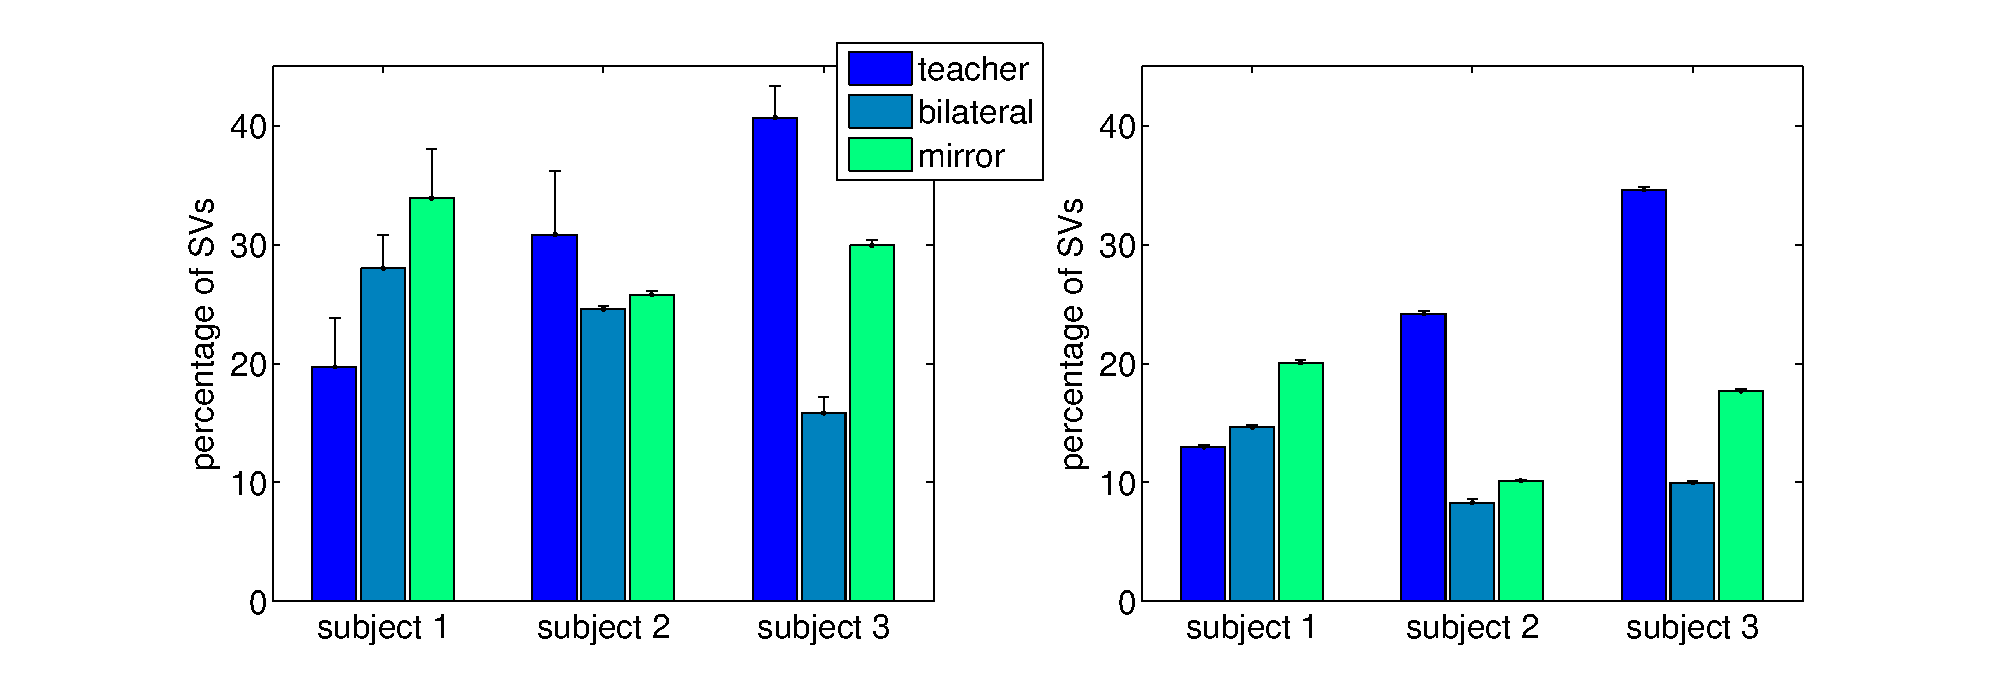
\includegraphics[width=\textwidth]{figs/figSVs}
  \caption{percentages of Support Vectors obtained in the optimal models
  	for classification (left) and regression (right) for each subject and modality.
    Histogram bars are mean values over the $10$ splits of
    the outer cross-validation, error bars denote one standard deviation.}
  \label{fig:SVs}
\end{figure*}
